% default font size and doc type
\documentclass[12pt]{article}

% extra packages to bring in
\usepackage{latexsym}
\usepackage{graphicx}      % extended graphics package
\usepackage{epsfig}        % wrapper for graphicx package
\usepackage{times}
\usepackage{url}
\usepackage{listings}
\usepackage{subcaption}

% margin settings borrowed from Dr. Teresco's example paper
\setlength{\topmargin}{-0.5in}
\setlength{\textheight}{9in}
\setlength{\oddsidemargin}{0in}
\setlength{\evensidemargin}{0in}
\setlength{\textwidth}{6.5in}

% single-space command borrowed from example paper
\newcommand{\singlespace}{
  \protect\renewcommand\baselinestretch{1.0}
  \protect\normalsize
}

% 1.5 spacing borrowed from example paper
\newcommand{\doublespace}{
  \protect\renewcommand\baselinestretch{1.5}
  \protect\normalsize
}


% begin typing document
\begin{document}

% remove date
\date{}

% paper title
\title{A Behavioral Approach to 6502 Emulation
\footnote{This work was completed in partial fulfillment of the final
project requirement for Computer Science 330 at Siena College, Fall 2020.}}

\author{M.~J.~Coppola, N.~S.~Shelby, L.~E.~Carleton\\
Computer Science 330\\
Siena College\\
Loudonville, NY, 12211
}

% make title
\maketitle
% remove page number from front page
\thispagestyle{empty}

% Abstract
\begin{abstract}
%The RP2A03 is the CPU found in the Nintendo Entertainment System (NES), launched October 18th, 1985.
%This processor was based off the MOS Technology 6502, differences being a lack of a decimal mode
%and the inclusion of the Audio Processing Unit (APU). Our goal is to create a partial implementation
%of an emulator for this CPU designed to be easily extended to a simple NES emulator.
An abstract goes here. We made a 6502 emulator that was partially implemented and easy to extend.
There were some results and we're really proud. Or something along those lines.
\end{abstract}

% double spacing
\doublespace
\section{Overview}
\label{sec:overview}
The RP2A03 is the CPU found in the Nintendo Entertainment System (NES), launched October 18th, 1985~\cite{nesdev_CPU, wikipediaNES}.
This processor was based off the MOS Technology 6502, differences being a lack of a decimal mode
and the inclusion of the Audio Processing Unit (APU)~\cite{nesdev_CPU}. Our goal is to create a partial implementation
of an emulator for this CPU designed to be easily extended to a simple NES emulator. 

The emulator was designed with the NES in mind. That being said, we only emulate the behavior of
the 6502, not precisely the actual hardware. This serves us a huge simplification in implementation.
Official operations of the 6502 only need to be calculated, and not emulated. We opted in for calculating
the output of the operations immediately, and then waiting the number of clock cycles that operation
took to execute.

Overview to be continued...

\section{Bitwise Operations}
\label{sec:bitwise}

Bitwise operations are major aspect of making an efficient emulator. Suppose we have an 8-bit value.
We typically express this value as a number, or possibly two hexidecimal digits. One way the 6502 uses
8-bit numbers is by defining parts of the binary expression as flags or smaller width values, shown in figure~\ref{fig:figure1}.
In emulation, it's important that we can extract information from this 8-bit number, as well as convert
information we already have into information we can store into this number. To achieve this, we use
bitwise operations.

% load figures
\begin{figure}[b!]
	\centering
	\begin{subfigure}[t]{0.5\linewidth}
		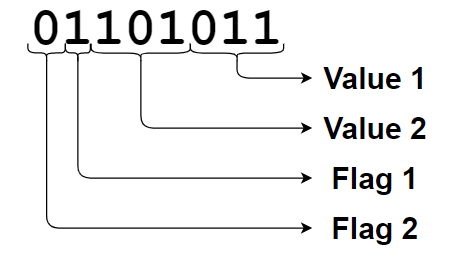
\includegraphics[bb=0 0 462 262]{figure1.PNG}
		\caption{A single binary value representing multiple values.}
		\label{fig:figure1}
	\end{subfigure}
	\begin{subfigure}[t]{0.4\linewidth}
		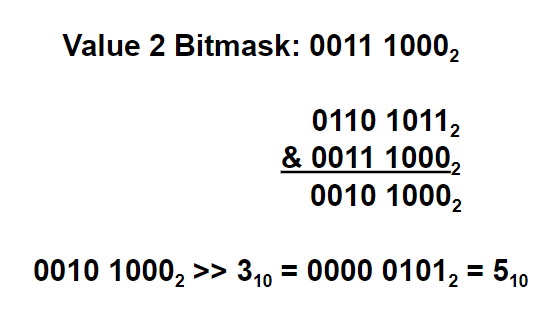
\includegraphics[bb=0 0 554 320]{figure2.PNG}
		\caption{Using a bitmask to extract values from a binary number.}
		\label{fig:figure2}
	\end{subfigure}
\end{figure}


To extract information from a binary number, we would first need to isolate that information using a bitmask.
We can create a bitmask by creating a new 8-bit number that has
1's placed over the important digits, and 0's on digits that are not. With this mask, we can use a
bitwise AND operation ( \lstinline{&} ) and have a result that only includes the digits defined by the bitmask shown in figure~\ref{fig:figure2}~\cite{bitmasks}.

In order to make this value useful to us, we may have to then use a bitwise shift-left ( \lstinline{>>} ) to push
the important digits to the least significant order of the digit. By doing this, the entirety of the
resulting 8-bit value numerically represents the value stored in the section of the original 8-bit
value~\cite{bitmasks}.

A similar process is used for setting bits as well. We create a bitmask for the bits we want to set
and or it with our value. To unset, we can \lstinline{&} with the inverse ( \lstinline{~} ) of our mask.
We can toggle/flip bits with a mask that is XOR'd ( \lstinline{^} ) with our value.

\section{NES Hardware}
\label{sec:neshardware}

\begin{figure}[h]
	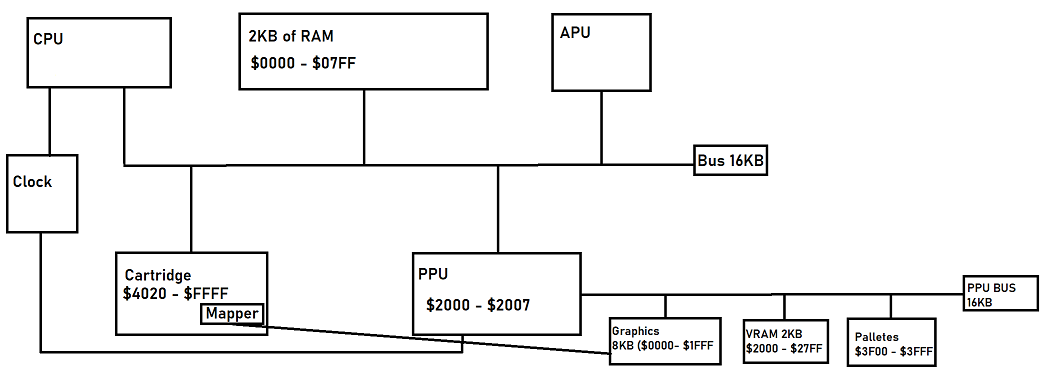
\includegraphics[width=2.0\linewidth,bb=0 0 1049 379]{NES_diagram.PNG}
	\caption{NES hardware bus diagram}
	\label{fig:nes_diag}
\end{figure}

The RP20A3 (6502) in the NES communicated to other devices on the machine using a 16-bit addressable
hardware bus. The CPU can read and write information to any device connected to the bus~\cite{mem_mapping}. 
Addresses \$0000 to \$00FF are mapped to the NES's 2KiB of internal memory. Parts of this memory has
predefined purposes dictated by the CPU architecture. The zero page is mapped to \$0000-\$00FF and the stack
is mapped to address \$0100 and onwards up to \$01FF~\cite{mem_mapping}. In our implementation, we map the entirtey of the
bus to read/write memory. A full NES implementation would have other devices on the bus.

The 6502 features 6 registers. The first major register is the 1-byte wide Accumulator (A) register.
This register is used with the ALU, and supports using the status register to describe its behavior,
such as denoting if its value is overflowing, negative, zero, etc. The X and Y registers are used for
different addressing modes. These registers were useful for looping when used with the increment and 
decrement instructions along side addressing with the value found in them. The program counter (PC) is a 
 2-byte wide register for tracking the current instruction in memory. The stack pointer register (S) is a 
1-byte wide register that holds the manipulatable value that points to the stack portion of memory. The
status (P) register hold 8 bytes (6 used) that store the current status flags of the CPU~\cite{cpu_registers}.

The 6502 has 3 index addressing modes. Addressing modes define where the CPU operations source operands
from. Zero page indexing uses a 1-byte address to find a value found in the hard-coded zero page.
We can offset the address to be read using the values in the X and Y register. Absolute addressing 
uses a 2-byte wide address to find memory outside of the zero page. Similarly, the X and Y registers
can be used to offset this address. The 6502 also features indirect addressing, which is it's solution
for simulating the function of pointers. The mode reads the value at the address found at the supplied
address. Unlike the previous addressing modes, the X and Y offsets server different purposes from
each other. The X register is used to offset the supplied address for the mode, while the Y register
is used to offset the value found at the supplied address~\cite{addressing_modes}.

Other addressing modes are also used. Many instructions operate directly on the accumulator. Others address
have immediate values from the program memory. Relative addressing is used by branching instructions
to move to a new instruction in program memory from -128 to 128 bytes away from the branch's address.

As instructions execute, the CPU updates the status register to reflect 6 different boolean flags. The
carry (C) flag turns on when an addition or subtraction carries or borrows a bit. This flag is also set if
a logic shift pushes out a 1.
The zero (Z) flag is turned on if an instruction results in a zero. The interrupt disable flag is used to enable and disable
maskable CPU interrupts. The overflow flag (V) is set when overflow is detected during an addition or subtraction,
and in a few other niche cases. The negative flag (N) is set when an instruction results in a negative value~\cite{status_flags}.

The first byte of an instruction is the opcode. Although only 56 opcodes are documented for the 6502,
there are 256 addressable opcodes in the CPU. The undocumented opcodes, known as illegal opcodes, usually
contain microcode the assist in the execution of the outward facing legal opcodes. An accurate emulator
will simulate the microcode, therefore the legal opcodes utilizing the microcode, as well as executing
them on the rare chance a developer uses one. Although a small subset of NES titles utilize these unofficial
opcodes, we will not implement them in the interest of time at the cost of 8 titles~\cite{illegal_ops}.

\section{Implementation}
\label{sec:implementation}

Our implementation begins with the bus. We decided to use a struct that can hold a bitfield
of several device memories that the CPU can access. Although our bus is capable of this, we opted
in for the bus to use memory in its entire address range as we will not be using any other devices.
The bus has only three simple functions for reading, writing and resetting the values in memory.
Our bus also can limit the range in which it can read and write data depending on what devices
are connected to it. With this limiter in code, we can change the behavior of the read/write depending on
the requested address range from the CPU.

To begin the CPU, we created an enumeration for all of the status flags of the CPU's status register.
Each flag in the enumeration holds the number 1 bitshifted to the location of the flag in the status register.
this allows us an easy way to refer to bitmasks as we set, unset, flip and test for status flags in the cpu.

We then created a structure to hold all of the CPU's information. The first component of the CPU is the 
registers. We used unsigned chars for each register, except for the program counter, which needs an unsigned short.
We added a get flag, and a set flag function to be able to easily test and write to the status register
in this CPU structure. In our structure, we include 5 helper values. We keep variables to store the current
observed address, the relative address used by branching instructions, the current opcode, how many
cycles are left needed to complete the current instruction and the fetched value from the addressing mode.

We also flesh out in put header file functions for our 12 addressing modes and 56 operations. We add
an extra opcode named XXX that captures all illegal opcodes. This serves as a no operation (NOP). We then
added a clock cycle function that performs 1 clock cycle in the CPU.

We created a structure the represents an instruction. This contains the name, the opcode, the addressing mode
and the number of cycles each type of instruction takes. With this structure, we can make a lookup table that
associates an opcode, structure and number of cycles each possible instruction takes based off the Rockwell instruction table
for the 6502~\cite{6502}.

Our addressing modes return the number of extra clock cycles the instruction takes, and the opcodes return
whether the operation takes an extra clock cycle. Using this information, the clock function can use the
lookup table to take an instruction, lookup the opcode in the lookup table, dereference and call the functions
found in the instruction structure it has found, and use those function return values to find out how many clock
cycles the operation took to execute.

\singlespace

\bibliographystyle{abbrv}
\bibliography{references}

% end document
\end{document}
